\documentclass[Setup/main.tex]{subfiles}

\pagenumbering{arabic}
\rfoot{
    \vspace{2 mm}
    Page \thepage \hspace{1pt} of 61
}
\begin{document}
\section{Introduction}

Efficiency, cost-effectiveness, and sustainability are essential in the fast-paced agricultural industry. Meeting the increasing demand for fresh, locally-grown produce requires innovation, and commercial gardeners are always searching for new ways to achieve this. Hydrovertic system is a modular solution that automates the manual process of transplanting plants from a block into separate cups, developed by experienced gardeners.

\begin{figure}[H]
    \centering
    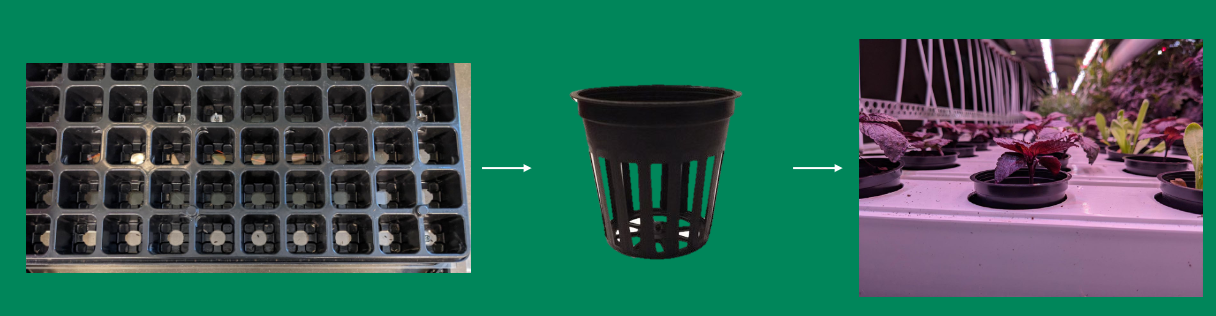
\includegraphics[width=\textwidth]{Tables and Images/problem_hydrovertic.jpg}
    \caption{Problem from Hydrovertic}
    \label{fig:problem}
\end{figure}


Automating the tedious process, as seen in figure \ref{fig:problem} of moving plants from modular blocks into tiny cups is the main goal of the HydroverticSystems project. This has always been a labor-intensive manual procedure that takes a lot of resources. This team has developed an automated idea to automate this process by using a robotic arm with a custom-designed gripper as a cutting-edge answer. The gripper has three main functions, transporting modular blocks around, picking a cup for the cupholder, and transposting a plant from the modular block to the cup. On top of that, a camera is used to detect the process of transporting the plant around and reporting any feedback about the overall process.

The advantages of Hydrovertic Systems are substantial. It boosts overall efficiency, accelerates production, and lowers labor expenses. Furthermore, it results in healthier and more fruitful crops by protecting every plant during the transplanting procedure. This introduction looks at the difficulties faced by commercial gardeners and the creative fix offered by Hydrovertic Systems. 


In the following sections, the overall process, development of the required tools, the implementation of the solution, and evaluation of the solution are going to be discussed. 


\end{document}

